\chapter[Learning Transports Without Losing Modes]{Learning Transports Without Losing Posterior Modes}
\label{ch:neutra-controlled-training}

A useful transport must reconcile two tasks. It must allocate probability to
the relevant regions of the posterior, and it must give Hamiltonian dynamics
coordinates in which numerical trajectories can move efficiently. Neither
task follows merely from a decreasing variational loss. The mixture examples
in Chapter~\ref{ch:rare-regions-transport} make this distinction measurable:
their probabilities and a reference transport are known, yet an estimated
transport can fit the centers of the modes while misrepresenting the valley.

Gaussianizing a posterior is stronger than covariance whitening. Centering
and scaling can give a multimodal distribution mean zero and identity
covariance while leaving its nonlinear score unchanged in character. On a
connected support equal to $\mathbb R^d$, the exact identity
$\nabla\log\pi_z(z)=-z$ instead implies
$\log\pi_z(z)+\|z\|^2/2$ is constant; normalization then identifies the
standard Gaussian density. A finite collection of score probes only tests
this identity at its sampled locations.

The appropriate response is to separate the sources of approximation. We first
establish that the sampler and its diagnostics work with a known transport.
We then distinguish error in the weighted training distribution from error in
fitting that distribution, and distinguish both from the effect of a subsequent
variational refinement. This ordering is particularly valuable when a long
sequence of repairs has changed several components at once.

\section[An exact transport control]{Separating learning from sampling}

Let $F_1$ be the cumulative distribution function of the first marginal in
\eqref{eq:rare-mixture-target}, and let $Z_1,Z_2$ be independent standard
normals. Define
\begin{equation}
 t(z_1)=F_1^{-1}(\Phi(z_1)),\qquad
 T(z)=\begin{pmatrix}t(z_1)\\z_2\end{pmatrix},\qquad
 T_w(z)=\begin{pmatrix}t(z_1)\\z_2+c(t(z_1)^2-26)\end{pmatrix},
 \label{eq:controlled-exact-transports}
\end{equation}
where $c=0.1$ for the warped benchmark. The derivative matrices are
\begin{equation}
 J_T=\begin{pmatrix}t'&0\\0&1\end{pmatrix},\qquad
 J_{T_w}=\begin{pmatrix}t'&0\\2ctt'&1\end{pmatrix}.
\end{equation}
Both determinants equal $t'$. Since $F_1(t(z_1))=\Phi(z_1)$,
$\pi_1(t)t'=\phi(z_1)$. The warped target evaluated at $T_w(z)$ equals
$\pi_1(t(z_1))\phi(z_2)$, because subtracting the warp recovers $z_2$.
Consequently,
\begin{equation}
 \pi(T(z))|\det J_T(z)|=\phi(z_1)\phi(z_2),\qquad
 \pi_w(T_w(z))|\det J_{T_w}(z)|=\phi(z_1)\phi(z_2).
 \label{eq:controlled-gaussian-pullback}
\end{equation}
The potential in these latent coordinates is quadratic and its score is $-z$.
The large marginal derivative at the valley therefore does not, by itself,
create a difficult exact latent target.

Numerical evaluation needs a separate check. A root finder locates $t$, but
differentiating its finite branch decisions is not the mathematical inverse
derivative. Implicit differentiation gives
\begin{equation}
 t'=\frac{\phi(z_1)}{\pi_1(t)},\qquad
 t''=t'\left[-z_1-(\log\pi_1)'(t)t'\right].
 \label{eq:controlled-inverse-derivatives}
\end{equation}
The second formula follows by differentiating $\log t'$. Logarithmic CDF and
survival-function comparisons avoid subtracting nearly equal tail
probabilities. A numerical check must compare the computed target-plus-log-
Jacobian expression and its derivative with
\eqref{eq:controlled-gaussian-pullback}; evaluating an analytic Gaussian
potential alone would bypass errors in that computation.

Three controls answer different questions: independent exact posterior samples
test the assessment procedure; Gaussian latent HMC with exact physical decoding
tests tuning and finite-run information; and the numerical change-of-variables
calculation tests transformation and differentiation. A failure of the latter
invalidates dependent numerical evidence. A stochastic diagnostic failure in
the former two requires assessment of its frequency and cause, rather than
an immediate declaration that the sampler is mathematically wrong.

The Gaussian control also makes trajectory resonances explicit. For unit
mass and potential $z^2/2$, one leapfrog step acts on position and momentum as
\begin{equation}
 \begin{pmatrix}z'\\v'\end{pmatrix}
 =M_\epsilon\begin{pmatrix}z\\v\end{pmatrix},\qquad
 M_\epsilon=
 \begin{pmatrix}
 1-\epsilon^2/2&\epsilon\\
 -\epsilon(1-\epsilon^2/4)&1-\epsilon^2/2
 \end{pmatrix}.
 \label{eq:controlled-gaussian-leapfrog}
\end{equation}
This follows by substituting the half momentum update into the position
update and then applying the second half momentum update. The determinant is
one, and for $0<\epsilon<2$ its eigenvalues are $e^{\pm i\omega}$ with
$\cos\omega=1-\epsilon^2/2$. At $\epsilon=1$, $\omega=\pi/3$:
lengths $L=3,9,18$ give $M_\epsilon^L=\pm I$, so position either alternates
sign or remains fixed, regardless of the refreshed momentum. High acceptance
cannot rescue these trajectories. At $\epsilon=\sqrt2$, the angle is
$\pi/2$, and $L=5,13,25$ all give the same matrix. Different trajectory
lengths therefore need not provide different Gaussian kernels.

There is also an exact stationary acceptance expression in this two-dimensional
control. Let $\lambda\geq1$ be the larger eigenvalue of
$(M_\epsilon^L)^\top M_\epsilon^L$; the other is $1/\lambda$. Under the
stationary joint position--momentum Gaussian law, rotational invariance gives
\begin{equation}
 2\Delta H=(\lambda-1)U-(1-\lambda^{-1})V,
 \qquad U,V\ \hbox{independent }\chi^2_2.
\end{equation}
To see the acceptance identity, append the usual momentum flip to the
leapfrog proposal and denote the resulting involution by $F$. Volume
preservation gives $dy=dx$ under $y=F(x)$, while
$e^{-H(x)}e^{-\Delta H(x)}=e^{-H(y)}$ and
$\Delta H(y)=-\Delta H(x)$. Thus the positive-energy part of the acceptance
integral equals the probability of a negative-energy proposal. Adding its
unit-acceptance negative-energy part gives
$\mathbb E\min(1,e^{-\Delta H})=2\Pr(\Delta H<0)$ when $\lambda>1$.
Since $U$ and $V$ are independent exponentials with the same scale,
$\Pr(U<V/\lambda)=\int_0^\infty e^{-\lambda u/2}
 e^{-u/2}\,du/2=1/(1+\lambda)$, and hence
\begin{equation}
 \mathbb E\alpha=\frac{2}{1+\lambda}.
\end{equation}
The formula extends continuously to acceptance one at $\lambda=1$.
For $\epsilon=\sqrt2$ and odd $L$, $\lambda=2$ and the expectation is
$2/3$. These identities explain the control's observed search behavior; they
do not determine acceptance for an imperfect learned map or establish
posterior precision. In particular, a nominal acceptance target does not
exclude a resonant or strongly correlated trajectory.

\section[The training distribution]{The weighted distribution actually supplied to the optimizer}

Suppose independent sampling replication $r$ supplies points $x_{ri}$ and
normalized weights $w_{ri}$, with $\sum_i w_{ri}=1$. Equal treatment of $R$
replications defines the empirical training measure
\begin{equation}
 \widehat\pi_R=\frac{1}{R}\sum_{r=1}^{R}\sum_iw_{ri}\delta_{x_{ri}},
 \qquad
 \widehat L_F(\theta)=-\frac{1}{R}\sum_{r,i}w_{ri}\log q_\theta(x_{ri}).
 \label{eq:controlled-pooled-teacher}
\end{equation}
A replication with more saved rows does not thereby receive more probability
mass. If each replication is self-normalized importance sampling, pooling
does not remove its finite-sample ratio bias. Replication labels remain useful
for estimating variability and identifying domination by one unusually
weighted run. For umbrella data, the window-normalization and overlap
requirements of \citet{thiede2016emus} remain necessary before this pooled
measure is meaningful.

For disjoint regions $B_k$, let $b_k=\widehat\pi_R(B_k)$ and let
$\widehat\pi_{R,k}$ be the normalized conditional empirical measure. If a
minibatch draws $n_k$ points from each conditional distribution, then
\begin{equation}
 \widehat\ell_F(\theta)
 =-\sum_k\frac{b_k}{n_k}\sum_{j=1}^{n_k}\log q_\theta(X_{kj}),
 \qquad X_{kj}\sim\widehat\pi_{R,k},
\end{equation}
has conditional expectation $\widehat L_F$. Allocating extra rows to the
valley improves its representation in individual updates without assigning
it a false posterior mass. Resampling the entire bank according to its tiny
valley mass would discard much of the information deliberately collected there.

The actual bank must be assessed on mode weights, conditional shape, and event
probabilities. A sampling method that passes across repeated runs does not
certify the particular replication later used for training. Conversely, a
correct empirical bank does not guarantee that the optimizer can fit it.
For the known mixture we can isolate these errors by constructing a separate
oracle bank: draw $U$ uniformly over each interval
$[F_1(a_k),F_1(a_{k+1})]$, set $X_1=F_1^{-1}(U)$, draw an independent
$X_2$, and attach the exact interval probability. Oracle-trained success is
evidence about fitting, not evidence that the estimated teacher works.
The conditional draws and stratum probabilities are exact in real arithmetic,
but their empirical bank is finite. This control removes uncertainty about
importance weights and stratum masses; it does not remove empirical
approximation within each stratum.

\section[Combined forward and reverse training]{Keeping example-based training during energy refinement}

\citet{noe2019boltzmanngenerators} combine maximum-likelihood training on
examples with energy-based training; their Methods equation~(9) permits both
terms, and supplementary Figure~S2 compares their effects on a double well.
This provides a direct source for testing joint forward and reverse objectives
without replacing the IAF architecture. In our notation,
\begin{align}
 L_F(\theta)&=-\mathbb E_\pi\log q_\theta(X),\\
 L_R(\theta)&=\mathbb E_{Z\sim\phi_d}
 \left[-\log\gamma(T_\theta(Z))-\log|\det J_{T_\theta}(Z)|\right],\\
 L_\lambda(\theta)&=L_R(\theta)+\lambda L_F(\theta),\qquad\lambda>0.
 \label{eq:controlled-joint-loss}
\end{align}
Using $q_\theta(T_\theta(z))=\phi_d(z)/|\det J_{T_\theta}(z)|$ and
$\pi=\gamma/\mathcal Z$, we obtain
\begin{align}
 \mathrm{KL}(q_\theta\|\pi)
 &=\mathbb E_{\phi_d}\log\phi_d(Z)+L_R(\theta)+\log\mathcal Z,\\
 \mathrm{KL}(\pi\|q_\theta)
 &=\mathbb E_\pi\log\pi(X)+L_F(\theta).
\end{align}
Thus $L_\lambda$ differs from
$\mathrm{KL}(q_\theta\|\pi)+\lambda\mathrm{KL}(\pi\|q_\theta)$ only
by constants independent of $\theta$. The unknown normalizer does not affect
its gradient. Replacing $\pi$ by \eqref{eq:controlled-pooled-teacher}, however,
replaces the forward expectation by an empirical one and introduces a distinct
approximation.

The forward loss reported by the optimizer is a cross entropy, so its absolute
level must not be read as a KL divergence. For these benchmarks its reference
level can be bounded almost exactly. Let $C$ denote the mixture label and put
$h_b(p)=-p\log p-(1-p)\log(1-p)$. The entropy identity for a discrete label
and a continuous observation gives
\begin{equation}
 h(\pi)=\log(2\pi e)+h_b(1/3)-H(C\mid X).
 \label{eq:controlled-target-entropy}
\end{equation}
The Bayes classification boundary is $t=-\log(2)/10$, obtained by equating
the two weighted marginal Gaussian densities. Its error probability is
\begin{equation}
 e_C=\tfrac13\Phi(-t-5)+\tfrac23\Phi(t-5)
     \simeq2.697\times10^{-7}.
\end{equation}
For the binary error indicator $E=\mathbf1\{C\ne\widehat C(X)\}$, knowing
$X$ and $E$ determines $C$. Therefore
$H(C\mid X)=H(E\mid X)\leq H(E)=h_b(e_C)$, while conditional entropy is
nonnegative. Substitution into \eqref{eq:controlled-target-entropy} yields
\begin{equation}
 3.4743868<h(\pi)<3.4743913.
\end{equation}
The warp has determinant one and hence preserves this entropy. A forward cross
entropy near $3.5003$ consequently corresponds to a forward KL near $0.0259$,
subject to the loss estimate's Monte Carlo error. This converts the units of
the reported loss; it does not certify either its gradient accuracy or its
sampling consequences.

This comparison also has an exact interpretation in the learned coordinates.
Let $\pi_{z,\theta}(z)=\pi(T_\theta(z))e^{d_\theta(z)}$, with
$d_\theta(z)=\log|\det J_{T_\theta}(z)|$. The density ratio obeys
\begin{equation}
 \frac{\pi(T_\theta(z))}{q_\theta(T_\theta(z))}
 =\frac{\pi_{z,\theta}(z)}{\phi_d(z)}.
\end{equation}
Changing variables in each KL integral therefore gives
\begin{equation}
 \mathrm{KL}(\pi\|q_\theta)
 =\mathrm{KL}(\pi_{z,\theta}\|\phi_d),\qquad
 \mathrm{KL}(q_\theta\|\pi)
 =\mathrm{KL}(\phi_d\|\pi_{z,\theta}).
 \label{eq:controlled-latent-kl}
\end{equation}
With exact expectations, the combined objective does seek a Gaussian latent
distribution in both KL directions. The unresolved issue is what these
integrated density errors imply about derivatives and finite HMC trajectories.
Replacing the forward expectation by a finite teacher bank weakens even that
population-level interpretation.

For a partition $B_k$, write $p_k=\pi(B_k)$, $v_k=q_\theta(B_k)$ and
$\pi_k=\pi(\cdot\mid B_k)$, $q_k=q_\theta(\cdot\mid B_k)$. On $B_k$,
$\pi/q_\theta=(p_k/v_k)(\pi_k/q_k)$, so substitution into the KL integral
gives
\begin{align}
 \mathrm{KL}(\pi\|q_\theta)
 &=\sum_k\int_{B_k}p_k\pi_k(x)
       \left[\log\frac{p_k}{v_k}+\log\frac{\pi_k(x)}{q_k(x)}\right]dx\\
 &=\sum_kp_k\log\frac{p_k}{v_k}
       +\sum_kp_k\mathrm{KL}(\pi_k\|q_k).
 \label{eq:controlled-kl-partition}
\end{align}
If a mode has $p_k>0$ while $v_k$ approaches zero, its forward penalty grows
without bound. Pure reverse KL does not impose this penalty: a proposal fitted
to the right component of the separated mixture has reverse KL close to
$-\log(2/3)$. Retaining the forward term therefore addresses a specific loss
of mode coverage. It does not eliminate nonconvex local optima or ensure
accurate derivatives in a region whose $p_k$ is extremely small.

The size of that penalty matters. For the broad valley, take the exact
probability $p=0.001349898$ and a proposal assigning $v=0.016$, almost twelve
times too much probability. Applying \eqref{eq:controlled-kl-partition} to the
event and its complement gives a forward mass contribution
$p\log(p/v)+(1-p)\log[(1-p)/(1-v)]\approx0.0114$ nats and a reverse mass
contribution of about $0.0250$ nats. Thus a seemingly small global KL can
coexist with a large relative error for a rare event. Stratified minibatches
reduce the variance of that event's gradient contribution, but correct
probability weighting leaves its expected contribution proportional to $p$.
Giving the event equal objective weight would change the objective; it would
not be a more accurate estimator of the same forward KL.

The author's double-well notebook retains unit weights for both ML and KL
after ML pretraining. We use $\lambda=1$ as that source-based baseline, not
as a universally optimal coefficient. The archived implementation also contains
an energy clipping transformation. Our analytic-target experiment omits that
transformation explicitly so that $L_R$ continues to use $\gamma$, rather than
a modified energy. Source fidelity requires identifying this difference.

The gradients must differentiate the same objectives. Define
$A_\theta(z)=\partial T_\theta(z)/\partial\theta$. With column gradients,
the ordinary reparameterized reverse gradient is
\begin{equation}
 \nabla_\theta L_R
 =-\mathbb E_{\phi_d}\left[
 A_\theta(Z)^\mathsf T\nabla_x\log\gamma(T_\theta(Z))
 +\partial_\theta d_\theta(Z)\right].
 \label{eq:controlled-reverse-gradient}
\end{equation}
Here $Z$ is held fixed while differentiating; interchange of differentiation
and expectation requires the usual integrability conditions. A value/score
interface to the target supplies $\nabla_x\log\gamma$, which equals the
posterior score because $\mathcal Z$ does not depend on the map parameters.

For a forward-training observation $x$, the physical point is fixed but its
inverse image $z_\theta=T_\theta^{-1}(x)$ changes. Implicit differentiation
of $T_\theta(z_\theta)=x$ gives
\begin{equation}
 \frac{\partial z_\theta}{\partial\theta}
 =-J_{T_\theta}(z_\theta)^{-1}A_\theta(z_\theta).
 \label{eq:controlled-parameter-inverse-derivative}
\end{equation}
Substituting this into the derivative of
$-\log\phi_d(z_\theta)+d_\theta(z_\theta)$ yields
\begin{equation}
 \nabla_\theta[-\log q_\theta(x)]
 =\partial_\theta d_\theta(z_\theta)
 -A_\theta(z_\theta)^\mathsf T J_{T_\theta}(z_\theta)^{-\mathsf T}
       [z_\theta+\nabla_z d_\theta(z_\theta)].
 \label{eq:controlled-forward-gradient}
\end{equation}
The partial derivatives on the right hold $z$ fixed; the second term supplies
the inverse map's dependence on $\theta$. Averaging this expression with the
corrected stratum weights gives the minibatch forward gradient. Treating the
training observations and their weights as fixed is appropriate, whereas
stopping the derivative through the inverse map would omit a required term.
As a sign check, in one dimension with $T_a(z)=az$ and $a>0$, the expression
reduces to $(1-z_a^2)/a$, the derivative of
$\log a+x^2/(2a^2)$ up to its constant.

The simultaneous gradient is
\begin{equation}
 g_\lambda=g_R+\lambda g_F.
\end{equation}
One Adam update using this sum is not generally equivalent to two successive
Adam updates, because Adam updates its first and second moments after each
gradient. Objective comparisons must also control whether those moments are
reset. We therefore distinguish preserved-state forward continuation from
reset-matched forward, reverse and combined branches starting at the same map.
The inverse-density evaluations in the forward term make their costs different;
equal numbers of updates are not equal computational effort.

\section[Optimization and geometry]{Optimization, capacity, and derivative accuracy}

An update limit is a computational allocation. To assess progress between
distinct maps $q_a,q_b$ on independent heldout points, define
$D_i=\log q_b(X_i)-\log q_a(X_i)$. The paired mean estimates the decrease
in forward cross entropy, and its uncertainty uses the variability of $D_i$,
not the separate variances of two unrelated estimates. Correlated chains and
weighted banks require block or replication uncertainty instead of an iid
standard error.

Failure to distinguish the mean from zero does not establish a plateau. A
practical plateau requires sufficiently precise evidence that further
improvement larger than a declared resolution is absent over the assessed
interval. That resolution remains an operational stopping choice. A run still
improving at its compute ceiling is under-budgeted, while a stationary poor
fit motivates an optimizer or capacity experiment. Neither outcome proves
that the IAF family cannot represent the target.

The conditional scale convention $s_j=b_j+c\tanh(h_j/c)$ bounds the nonlinear
log-scale contribution, but does not bound every conditioner derivative or
off-diagonal Jacobian term. The score residual from
\eqref{eq:rare-pullback-score} should therefore be inspected on Gaussian-base
points, independent posterior points pulled back through the map, and directed
physical points spanning several valley slices. These sampling measures answer
different questions. A finite maximum is not a uniform bound.

The residual has a useful second expression. The density induced by the map
satisfies
\begin{equation}
 \log q_\theta(T_\theta(z))+\log|\det J_{T_\theta}(z)|
 =\log\phi_d(z).
\end{equation}
Differentiating with respect to $z$ and subtracting the resulting identity
from the transformed posterior score gives
\begin{equation}
 r_\theta(z)=J_{T_\theta}(z)^\mathsf T
 \left[\nabla_x\log\pi(x)-\nabla_x\log q_\theta(x)\right]_{x=T_\theta(z)}.
 \label{eq:controlled-score-error-amplification}
\end{equation}
Thus the residual depends on both the physical density's score error and the
map's stretching in the direction of that error. The bound
$\|r_\theta\|\leq\|J_{T_\theta}\|_2
\|\nabla\log\pi-\nabla\log q_\theta\|$ makes the sensitivity explicit.
For example, stretching of $2.4\times10^5$, comparable to the exact marginal
transport at the valley center, would amplify a score error of $10^{-3}$
aligned with that direction to a residual of about $240$. This illustrates
sensitivity; it is not a measurement of either factor for a particular fitted
map. The exact map itself has zero score error and zero residual.

The counterexample in \eqref{eq:rare-kl-score-counterexample} explains why
derivative checks remain necessary even when both KL objectives are small.
An alternative perturbation gives explicit rates for both divergences.
Consider the following smooth density in one latent coordinate, with $k>1$
and $a_k=k^{-1/2}$:
\begin{equation}
 p_k(z)=\phi(z)\{1+a_k\sin(kz)\}.
 \label{eq:controlled-small-kl-density}
\end{equation}
It is positive, and it integrates to one because the Gaussian is even and
the sine is odd. Put $u=a_k\sin(kz)$. The inequality $\log(1+u)\leq u$
and $\mathbb E_\phi u=0$ give
\begin{equation}
 \mathrm{KL}(p_k\|\phi)
 =\mathbb E_\phi[(1+u)\log(1+u)]
 \leq\mathbb E_\phi(u+u^2)\leq a_k^2.
\end{equation}
For the other direction, Taylor's theorem applied to $-\log(1+u)$ gives
$-\log(1+u)\leq-u+u^2/[2(1-a_k)^2]$, since $|u|\leq a_k<1$.
Therefore
\begin{equation}
 \mathrm{KL}(\phi\|p_k)\leq\frac{a_k^2}{2(1-a_k)^2}.
\end{equation}
Both divergences tend to zero. Yet its Gaussian score residual is
\begin{equation}
 r_k(z)=\frac{d}{dz}\log p_k(z)+z
       =\frac{a_k k\cos(kz)}{1+a_k\sin(kz)}.
\end{equation}
Using $\mathbb E_\phi\cos^2(kZ)=(1+e^{-2k^2})/2$, we obtain
\begin{equation}
 \mathbb E_\phi r_k(Z)^2
 \geq \frac{a_k^2k^2}{2(1+a_k)^2}(1+e^{-2k^2})
 \longrightarrow\infty.
 \label{eq:controlled-kl-score-counterexample}
\end{equation}
Small, rapidly varying density errors can thus have large derivatives. For
example, $k=10^6$ and $a_k=10^{-3}$ give upper bounds of $10^{-6}$ for both
KL divergences, while the residual RMS exceeds $700$. This counterexample
does not identify the cause of a particular trained map's error. It shows
why minimizing a sum of forward and reverse KL, by itself, cannot guarantee
accurate scores without additional regularity or derivative evidence.

\begin{figure}[htbp]
 \centering
 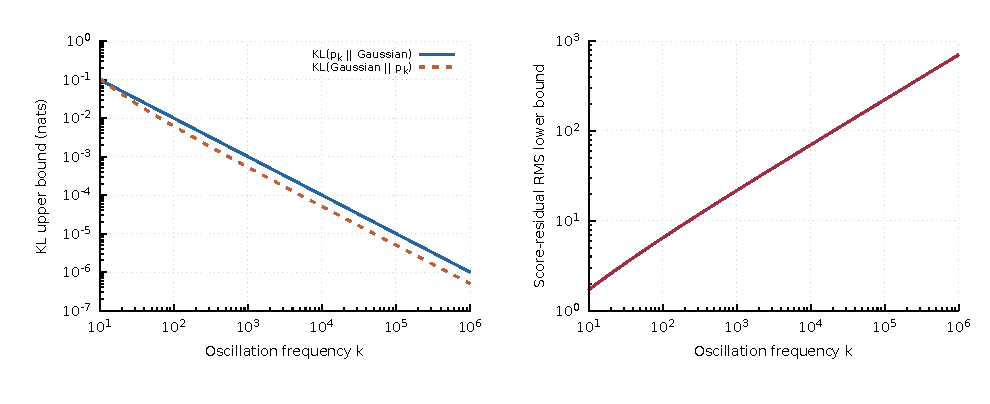
\includegraphics[width=\textwidth]{figures/neutra_kl_score_bounds.pdf}
 \caption{Deterministic bounds for \eqref{eq:controlled-small-kl-density}.
 Both KL upper bounds decrease with oscillation frequency, while the lower
 bound on Gaussian score-residual RMS grows. The right panel drops the
 positive $e^{-2k^2}$ term in \eqref{eq:controlled-kl-score-counterexample},
 retaining a valid lower bound. These are mathematical bounds, not fitted
 transport results.}
 \label{fig:controlled-kl-score-bounds}
\end{figure}

If density fits are adequate but derivative errors remain harmful, an optional
geometric objective can be derived. For fixed physical reference measures
$\nu_k$ and declared nonnegative coefficients $a_k$, consider
\begin{equation}
 G(\theta)=\sum_k a_k\mathbb E_{X\sim\nu_k}
   \left[\|r_\theta(T_\theta^{-1}(X))\|^2\right].
 \label{eq:controlled-geometric-objective}
\end{equation}
Writing $\delta s_\theta(x)=\nabla\log\pi(x)-\nabla\log q_\theta(x)$,
put $z_\theta=T_\theta^{-1}(x)$ and $J_\theta=J_{T_\theta}(z_\theta)$.
Equation~\eqref{eq:controlled-score-error-amplification} expresses the
integrand as
\begin{equation}
 \|r_\theta(z_\theta)\|^2
 =\delta s_\theta(x)^\mathsf T J_\theta J_\theta^\mathsf T
      \delta s_\theta(x).
\end{equation}
It therefore weights physical score errors by a metric that also changes with
the fitted map.
This is an explicit local extension, not the original NeuTra training
prescription. The inverse derivative in
\eqref{eq:controlled-parameter-inverse-derivative} remains necessary: the
derivative of the residual includes both its explicit parameter dependence
and its change through $z_\theta$. Dropping the latter
term computes a different derivative. The physical score at fixed $x$ can be
stored. More explicitly, the total derivative of the residual is
\begin{equation}
 B_\theta(x)
 =\partial_\theta r_\theta(z_\theta)
  -[\partial_z r_\theta(z_\theta)]
       J_{T_\theta}(z_\theta)^{-1}A_\theta(z_\theta).
\end{equation}
Applying the derivative of a squared norm then gives
\begin{equation}
 \nabla_\theta G
 =2\sum_k a_k\mathbb E_{\nu_k}
       [B_\theta(X)^\mathsf T r_\theta(T_\theta^{-1}(X))],
 \label{eq:controlled-geometric-gradient}
\end{equation}
provided differentiation can be interchanged with these fixed-measure
expectations. The matrix $B_\theta$ has one row per residual coordinate and
one column per parameter; its second term accounts for keeping the physical
point fixed as the map changes. Mixed and higher derivatives of the map still
need numerical and computational validation before such an objective is
useful. For a scalar check, take $T_a(z)=az$, $a>0$, and a target
$N(0,\tau^2)$. Then $r_a(z)=(1-a^2/\tau^2)z$, so at fixed $x$
the residual is $x/a-ax/\tau^2$ and its derivative is
$B_a(x)=-x/a^2-x/\tau^2$. Holding $z$ fixed would instead give
$-2x/\tau^2$, missing the required inverse dependence. These expressions
apply where the required derivatives exist. With the canonical unit-parameter
ELU, the first derivative is continuous at zero but the second derivative has
different one-sided limits. Tests of an implemented geometric objective would
therefore need to distinguish ordinary differentiable points from activation
boundaries; a single directional check at a smooth point would not settle its
behavior at every such boundary.

The reaction-coordinate entropy objective in
\citet{noe2019boltzmanngenerators} has a different purpose: it deliberately
encourages sampling of high-energy transition configurations. Exact correction
can recover posterior expectations from an appropriate proposal, but spreading
proposal mass along a reaction coordinate is not the same as making the
posterior pullback Gaussian. These mechanisms should be tested separately.

\section[Sampling and confirmation]{Evidence from posterior computation}

For a frozen proposal density $q$, an independence proposal is accepted with
probability
\begin{equation}
 \alpha(x,y)=\min\left\{1,\frac{\gamma(y)q(x)}{\gamma(x)q(y)}\right\}.
\end{equation}
This permits global jumps without requiring the proposal to equal the target.
\citet{gabrie2022adaptiveflows} combine such moves with local exploration and
discuss mixtures of separately trained maps. If two fixed kernels preserve
$\pi$, their composition preserves $\pi$ because $\pi K_1K_2=\pi K_2=\pi$;
the composition need not itself satisfy detailed balance. These fixed-kernel
identities do not prove convergence of an arbitrary finite adaptive run.
Training-sample collection must distinguish adapting exploration from frozen,
assessed sampling.

For NeuTra HMC, the frozen map is used with the exact transformed target and
identity latent mass. Independent verification of a step-size/trajectory pair
precedes posterior assessment. Known mode locations can supply a separate
start bank with within-mode variation; they are not posterior samples. Agreement
of chains started entirely within one learned component does not test the
missing component. Final confirmation must also use fresh streams after map
selection.

For a stationary event indicator with integrated autocorrelation time $\tau_A$,
the Markov-chain central limit approximation is
\begin{equation}
 \operatorname{Var}(\widehat a)\simeq\frac{a(1-a)\tau_A}{N},\qquad
 N_{\mathrm{eff},A}=N/\tau_A,
 \qquad
 \frac{\operatorname{MCSE}(\widehat a)}{a}
 \simeq\sqrt{\frac{1-a}{aN_{\mathrm{eff},A}}}.
 \label{eq:controlled-event-precision}
\end{equation}
This assumes a suitable central limit theorem and an estimable autocorrelation
sum; a trace with few events cannot validate those assumptions merely by
returning a finite ESS. For the broad valley, a 20 percent relative MCSE needs
about $18{,}500$ independent-equivalent observations, and 10 percent needs about
$74{,}000$. Four chains capped at $10{,}000$ retained draws each therefore do
not routinely support the latter goal. The much rarer central event remains
a task for deliberate estimators rather than an ordinary-HMC observation gate.

\citet{hoffman2019neutra} explicitly note that an inadequate map can slow tail
mixing. A failed frozen-map run can accordingly indicate poor coordinates,
inadequate kernel search, or insufficient retained information. It does not
prove an incorrect invariant distribution. Conversely, a valid invariant
distribution alone does not establish an accurate finite posterior estimate.

\section[Implementation and evidence]{Implementation and recorded evidence}

The controlled experiment retains the shared canonical IAF implementation and
uses one checked Adam update for the combined objective. It preserves
parameters, optimizer moments, iteration counts, teacher identity and unique
random streams at checkpoints. Exact references, estimated teachers and
learned-map results are stored separately. The controller refreshes its next
phase after each result: continuing progress receives further budget,
teacher failure receives a bounded sampling repair, an optimizer plateau
receives a declared capacity or learning-rate experiment, and an inconclusive
kernel search receives its declared wider search. An invalid common reference
stops dependent work.

The experiment crosses the two targets with oracle and importance-weighted
teachers and development seeds $11$ and $37$. The architecture has three
canonical IAF stages and two ELU hidden layers per stage. Each parent uses a
$1{,}024$-update pilot at widths $16$ and $32$ and learning rates
$3\times10^{-4}$ and $10^{-3}$ to nominate a configuration by heldout forward
loss. That nomination allocates subsequent training; it does not establish
posterior quality. The kernel initializer's variance-scale multiplier $0.2$
is a previously investigated local training choice, distinct from the author's
$0.02$ choice. The optimizer
uses batches of $256$, Adam coefficients $(0.9,0.999)$ and numerical offset
$10^{-8}$, with no gradient clipping. These inherited optimizer choices remain
hypotheses for these targets. The ordinary training rungs are $2{,}048$,
$8{,}192$ and $32{,}768$ updates; continuation preserves its declared ancestor
and optimizer state. The combined branch uses $\lambda=1$.

All numerical work here uses TensorFlow/TFP with XLA and FP64 as a diagnostic
reference. The experiment does not evaluate the intended FP32/TF32 training
policy. The teacher arms follow the same pilot protocol but can select different
widths and learning rates, so their comparison does not isolate teacher quality
at a fixed architecture and optimizer. Within a case the objective branches
share their initial fitted map. Their costs differ, and the two development
seeds do not support a statistical ranking of objectives. Hardware is shared
with other workloads; the recorded process times account for resource use but
do not establish device throughput.

The numerical exact-transport checks on both targets used $1{,}001$ directed
points. Maximum errors were $3.6\times10^{-15}$ in log density,
$3.6\times10^{-10}$ in score, and $2.3\times10^{-16}$ in marginal probability.
Eight independent iid streams, paired across the two targets, passed the
declared retained-sample and reference checks in all sixteen evaluations.
The Gaussian HMC control passed on both targets after the resonance and
finite-information repairs described above. The passing run used
$\epsilon=1.6817928305$, $L=5$, $2{,}000$ discarded warm-up draws and
$9{,}000$ retained draws per chain. Its broad-event relative MCSE was about
$18.9$ percent. These finite controls establish feasibility for this
experiment; their small replication count does not calibrate a general
false-rejection rate or nominal sequential coverage.

The first oracle-teacher fit illustrates why the learning question remains
separate. After $32{,}768$ forward updates, the median Gaussian-base residual
was $0.312$, but the maximum over the directed valley slices was about $433$.
That maximum is descriptive, and the measured forward objective was still
improving. Subsequent pure reverse and combined refinements therefore cannot
be interpreted as comparisons of globally optimized densities. Joint training
and its preserved-Adam continuation brought the selected map to $131{,}072$
lifetime updates, including its forward-trained ancestor. Its estimated reverse
KL was $0.0299$ and its Gaussian-probe median residual was $0.168$, but the
directed maximum was about $1{,}181$; Figure~\ref{fig:controlled-valley-residuals}
shows the latter diagnostic across the valley. The same $1{,}000$ Gaussian
probes had a mean residual norm of $6.39$, a 99th percentile of about $102$,
and a maximum of about $1{,}029$. Thus the low median concealed substantial
errors already visible in the ordinary probe bank. These tail summaries are
descriptive and are not precise estimates of population extreme quantiles.
The last paired joint-objective
gain was $0.00476$ with standard error $0.00746$, which did not establish the
declared operational plateau. The bounded HMC procedure failed to qualify this
case. A subsequent completion pass excluded the already completed failed
kernel and assessed three remaining verified settings at the same retained
cap. Each produced $40{,}000$ retained draws in total; their broad-valley
counts were $1$, $8$, and $15$, compared with approximately $54$ expected
visits for $40{,}000$ stationary draws. The expected count uses linearity of
expectation, but its sampling variation depends on serial dependence; a
binomial uncertainty calculation would not be justified for these chains.
All three failed the declared event checks, with estimated relative MCSEs
of approximately $100$, $68$, and $55$ percent. Such sparse counts also make
the MCSE estimates fragile. The operational conclusion is that these kernels
did not deliver the specified finite-sample event accuracy. Neither these
residuals nor the incomplete optimization justify a claim
that the IAF family cannot solve the problem.

\begin{figure}[htbp]
 \centering
 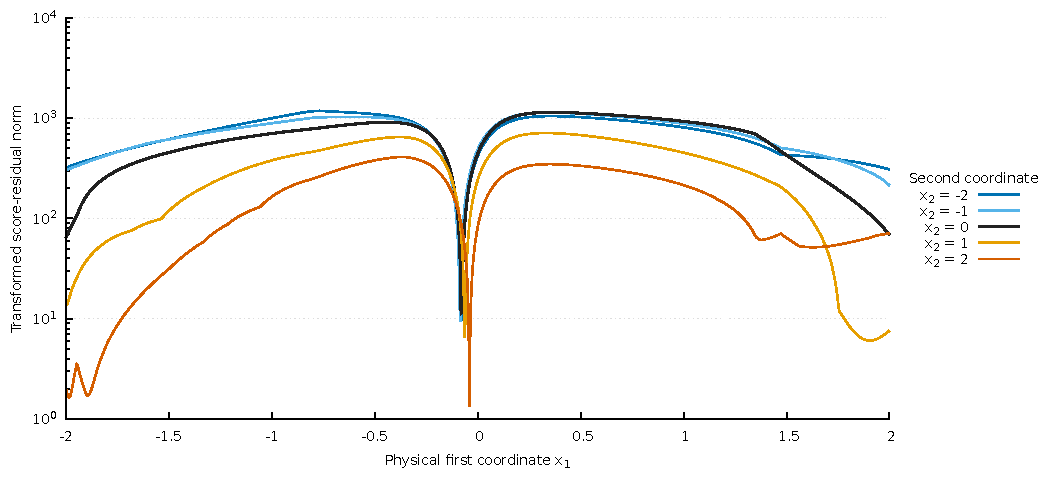
\includegraphics[width=\textwidth]{figures/neutra_controlled_valley_residuals.pdf}
 \caption{Directed score residuals for the first oracle-mixture case after
 joint training and continuation. Each curve fixes the physical second
 coordinate and evaluates $1{,}001$ locations across the valley. These points
 were deliberately placed; their norms are not a posterior error distribution
 or a uniform bound. The figure reads the saved FP64 diagnostics of the
 $131{,}072$-lifetime-update map and makes no comparison of methods.}
 \label{fig:controlled-valley-residuals}
\end{figure}

The completed training phase comprised $48$ fit jobs across the eight
target--teacher--seed cases. All stopped at their work allocations; none
established the operational plateau. Table~\ref{tab:controlled-final-maps}
records the final joint checkpoints, including their one continuation. The
within-case objective branches and earlier checkpoints remain in the full
result record. This table describes the final maps; it does not rank them or
select them for posterior use.

\begin{table}[htbp]
 \centering\small
 \begin{tabular}{llrrrrr}
 \toprule
 Target & Teacher & Seed & \shortstack{Lifetime\\updates} &
 \shortstack{Estimated\\reverse KL} & \shortstack{Median\\residual} &
 \shortstack{Directed\\maximum}\\
 \midrule
 Unwarped & Oracle & 11 & 131072 & 0.0299 & 0.168 & 1181\\
 Unwarped & Oracle & 37 & 73728 & 0.0255 & 0.156 & 3702\\
 Unwarped & Estimated & 11 & 73728 & 0.0205 & 0.135 & 4873\\
 Unwarped & Estimated & 37 & 73728 & 0.0084 & 0.103 & 3286\\
 Warped & Oracle & 11 & 24576 & 0.0253 & 0.222 & 1563\\
 Warped & Oracle & 37 & 106496 & 0.0101 & 0.117 & 3635\\
 Warped & Estimated & 11 & 131072 & 0.0210 & 0.091 & 4124\\
 Warped & Estimated & 37 & 131072 & 0.0261 & 0.150 & 1673\\
 \bottomrule
 \end{tabular}
 \caption{Final joint maps from the FP64 controlled experiment. The median
 uses the standard $1{,}000$ Gaussian-base probes; the maximum uses five
 directed physical valley slices. These are different sampling measures.
 Reverse KL estimates use a separate finite Gaussian bank. All values are
 descriptive; posterior qualification is assessed separately.}
 \label{tab:controlled-final-maps}
\end{table}

Four continuations completed only one new checkpoint, leaving no within-job
paired loss change. Among those with multiple new checkpoints, the last
joint-loss standard errors ranged from about $0.0035$ to $0.0078$ nats,
larger than the $0.001$-nat plateau resolution even before the three-standard-
error margin. This is inconclusive optimization evidence. It does not support
the prerequisite for the optional geometric objective, which was therefore
neither implemented nor executed in this campaign. Its derivation above is a
proposal for a distinct experiment.

The complete posterior execution record belongs in the accompanying campaign
result note. The substantive success criterion remains a finite posterior
computation that passes the declared physical-space accuracy and information
requirements, together with its measured computational cost and limitations.

In the completed eight-case campaign, no learned map passed fresh posterior
confirmation. The exact transport, independent-reference and exact Gaussian
controls passed for both targets, so the result is a failure of the bounded
learned-map training and sampling procedure under this evidence contract. The
fit failures cannot be attributed solely to importance-weight estimation,
because the exact conditional oracle teacher also failed. At the same time,
all forty-eight fit jobs stopped at their work allocations, and the plateau
criterion was never established. Incomplete optimization, capacity, local
geometry and finite HMC information therefore remain competing explanations.
The optional geometric objective was not executed; its prerequisite of an
adequate stationary density fit was not demonstrated.

\section[What the subsequent fits identify]{What the subsequent exact-sample fits identify}
\label{sec:neutra-october-fit-attribution}

The subsequent experiment on randomized two- and three-component Gaussian
mixtures isolates a failure that occurs even before an approximate sampler
supplies the training data. Its four independent exact-sample banks contain
$4{,}096$ observations in total. The forward fit resamples these observations
with their empirical probabilities, so its expected minibatch gradient is
the gradient of the empirical forward cross entropy. Exact sampling removes
an approximate sampler as the cause of this failure; it does not remove
finite-data error or establish that the optimizer reaches the population
optimum.

In the October 4 experiment, both widths, $32$ and $64$, retained three IAF
stages. They received $4{,}096$ and $8{,}192$ forward updates respectively,
followed by $256$ reverse-KL updates with a fresh Adam state. The objective
switch occurred regardless of the forward assessment. Changing width and
update count together prevents this comparison from identifying a width
effect. Moreover, the learning histories did not establish a stationary
forward optimum. All four final maps failed the declared distribution screen,
and the native teacher experiments consequently did not run.

Checks of the eight saved forward and final maps found inverse and
log-determinant discrepancies of approximately $10^{-14}$ and directional
parameter-derivative discrepancies up to $1.29\times10^{-7}$ in the
checked FP64 reference calculations. No gradient clipping occurred during
these fits, and the sampled conditional-scale diagnostics did not show strong
cap saturation. These observations weaken specific explanations based on
incorrect local derivatives or clipping. They do not prove every execution
path correct, establish sufficient capacity, or validate the complete
training procedure.

The forward maps already assigned excessive mass away from the components.
For a two-dimensional Gaussian mixture
$p(x)=\sum_{k=1}^K w_k\varphi_k(x)$, let
$d_k^2(x)=(x-\mu_k)^\mathsf T\Sigma_k^{-1}(x-\mu_k)$ and define
\begin{equation}
 E=\{x:d_k^2(x)>8\ \text{for every }k\}.
\end{equation}
Conditional on component $k$, this event is contained in
$\{d_k^2(X)>8\}$. Since a component's squared Mahalanobis distance is
$\chi^2_2$, the exact target therefore satisfies
\begin{equation}
 p(E)=\sum_k w_k\Pr_{\varphi_k}(E)
 \leq\sum_k w_k e^{-4}=e^{-4}\simeq0.01832.
 \label{eq:neutra-mixture-ellipse-bound}
\end{equation}
The width-$64$ forward maps assigned approximately $8.39$ percent and
$21.62$ percent to this event for the two- and three-component targets.
These estimates use $32{,}768$ new Gaussian-base draws per target. Their
uncertainty concerns numerical integration for fixed fitted maps, rather
than variability across repeated training runs. The bound is an upper
bound on target mass, not a formula for its exact value.

The subsequent coverage loss has an exact reverse-KL interpretation that
does not require disjoint Gaussian components. Define the target
responsibilities and the learned responsibility masses by
\begin{equation}
 r_k(x)=\frac{w_k\varphi_k(x)}{p(x)},\qquad
 a_k=\int q(x)r_k(x)\,dx,\qquad
 q_k(x)=\frac{q(x)r_k(x)}{a_k}.
\end{equation}
Here $q_k$ is the conditional density induced by assigning target
responsibilities to draws from $q$; it is not assumed to be Gaussian.
The augmented densities
$\widetilde p(x,k)=p(x)r_k(x)=w_k\varphi_k(x)$ and
$\widetilde q(x,k)=q(x)r_k(x)=a_kq_k(x)$ have ratio $q(x)/p(x)$.
Summing the augmented KL over $k$ therefore leaves the marginal KL
unchanged and yields
\begin{align}
 D_{\mathrm{KL}}(q\|p)
 &=\sum_k\int a_kq_k(x)
       \log\frac{a_kq_k(x)}{w_k\varphi_k(x)}\,dx\\
 &=\sum_k a_k\log\frac{a_k}{w_k}
   +\sum_k a_kD_{\mathrm{KL}}(q_k\|\varphi_k).
 \label{eq:neutra-responsibility-kl-decomposition}
\end{align}
The first term penalizes incorrect component allocation. The second
penalizes conditional shape error, weighted by the probability that the
learned density itself assigns to that component.

\begin{table}[htbp]
 \centering
 \begin{tabular}{lrr}
  \toprule
  Quantity, width-$64$ three-component fit & Forward endpoint & After RKL\\
  \midrule
  Second responsibility mass $a_2$ & $0.21572$ & $0.02240$\\
  Allocation KL & $0.00319$ & $0.20984$\\
  Weighted conditional-shape KL & $1.69401$ & $0.41727$\\
  Total reverse KL & $1.69721$ & $0.62711$\\
  Heldout forward KL & $0.42979$ & $1.14216$\\
  \bottomrule
 \end{tabular}
 \caption{The objective switch reduces reverse KL while worsening coverage.
 The target second-component weight is $0.249591$. Estimates describe one
 pair of fixed checkpoints; they do not rank training methods.}
 \label{tab:neutra-objective-switch-attribution}
\end{table}

Table~\ref{tab:neutra-objective-switch-attribution} shows that the reduction
in weighted shape cost exceeds the increase in allocation cost. With common
integration draws, the change in $a_2$ is $-0.19333$, with an approximate
$95$ percent integration interval $[-0.19753,-0.18913]$. The reverse-KL
change is $-1.07010$, with estimated integration standard error $0.03867$.
Thus this coverage regression is compatible with correctly computed
reverse-KL optimization. It does not show that reverse KL always loses modes.
The poor forward endpoints also show why simply omitting the reverse stage
would leave a substantial fitting problem.

\section[Published remedies]{Remedies in the literature}
\label{sec:neutra-literature-remedies}

The combined objective in \eqref{eq:controlled-joint-loss} has a direct
precedent in \citet[][Methods, Eq.~(9)]{noe2019boltzmanngenerators}.
Their original double-well notebook performs maximum-likelihood pretraining
and then retains both maximum-likelihood and energy terms. Similarly,
\citet[][Sec.~III.B and Appendix~A.2]{gabrie2022adaptiveflows} describe
combining the two objectives after a sufficiently accurate forward fit.
Equation~\eqref{eq:controlled-kl-partition} explains the protection that
the forward term supplies: eliminating a region with positive target mass
has an unbounded forward penalty. Finite weights, finite examples and
nonconvex optimization still permit substantial error. In particular, the
earlier eight-case experiment in this chapter already tried joint and
joint-continuation training without attaining fresh posterior confirmation.
The literature supports testing this mechanism carefully; it does not make
it a previously untried or sufficient cure for the present failure.

Representation is a separate choice. A scalar affine transformation of a
Gaussian remains Gaussian at fixed conditioning variables. The nonlinear
monotone transformations of \citet[][Sec.~3 and Fig.~5]{huang2018naf}
can instead create multiple scalar density peaks through changes in their
derivative. Composing and permuting affine autoregressive stages can also
produce complex multivariate densities, so this distinction is not a proof
that the current IAF family cannot represent the mixture. It identifies a
reason to compare representations after controlling optimization effort.
The Gaussian mixtures considered here are positive throughout
$\mathbb R^d$; an impossibility argument based on disconnected support does
not apply to them. The exact transport in
\eqref{eq:controlled-exact-transports} is also a constructive reminder that
Gaussianization and numerical ease of learning that Gaussianization are
different questions.

\citet[][Sec.~3.1, Eqs.~(4)--(8)]{durkan2019splines} offer a useful
computational alternative. Their monotone rational-quadratic scalar splines
have analytic derivatives and inverses. In an autoregressive construction
the Jacobian remains triangular, with
\begin{equation}
 \log|\det J_T(z)|
 =\sum_j\log\left|\frac{\partial T_j(z)}{\partial z_j}\right|.
\end{equation}
The inverse within a spline bin follows from a quadratic equation, as in
the original implementation. This avoids a dense determinant, although an
autoregressive inverse can still require sequential coordinate evaluation.
The usual splines are continuously differentiable; regularity of the
transformed force at knots requires separate attention for HMC. Such a
comparison would evaluate an explicitly different map family, rather than
silently redefining the canonical IAF.

\citet[][Sec.~IV.E]{gabrie2022adaptiveflows} also recommend informed base
distributions, appropriate coordinate scaling and mixtures of maps fitted
to different modes. Their Gaussian-mixture experiment uses six pairs of
RealNVP coupling layers with width-$100$ conditioners. It is therefore not
an experiment with our three-stage IAF. Appendix~G.1 reports a residual
connection between modes even in the successful example and states that
additional training would make it thinner. The proposed mixture-of-maps
strategy reduces the burden on any individual map, but produces a mixture
proposal, not automatically a single invertible Gaussian coordinate chart
for the existing NeuTra HMC procedure.

Fresh training information addresses another failure mechanism. Gabri\'e's
Algorithm~1 alternates local moves, global flow proposals and forward
training. Local moves explore details the flow misses, while accepted
global proposals help adjust relative mode weights. Section~IV.C assumes
initial representatives of the relevant modes; the method does not promise
to discover every unrepresented basin. Moreover, the paper's ULA experiments
retain discretization error, even though corrected MALA is available in the
algorithm. Fixed-kernel invariance and convergence of a finite adaptive
implementation must be assessed separately.

Annealed flow transport divides a difficult transformation into transitions
between intermediate distributions. The practical AFT procedure of
\citet[][Sec.~3.3 and Appendix~F]{arbel2021aft} uses training, validation
and test populations to limit overfitting and separate fitting from
evaluation. \citet[][Sec.~2.3]{matthews2022craft} identify the remaining
sample-replenishment problem: repeatedly optimizing on one finite
population can exhaust the information available for learning a flow.
CRAFT uses repeated annealed passes with fresh initial particles and retains
importance, resampling and Markov corrections. Its finite-particle gradient
is not generally an unbiased gradient of the exact-target objective;
Section~3.2 instead gives an unbiased-gradient interpretation for a modified
objective involving the expected finite-particle distribution. These methods
improve the sampling-and-learning procedure, but cannot alone explain or
repair failure of a separate student already supplied with exact samples.

FAB strengthens the penalty for missed mass through an objective
proportional to $\int p(x)^2/q(x)\,dx$, with AIS targeting its normalized
integrand \citep[][Sec.~3.1]{midgley2023fab}. The method concentrates effort
where the target density is appreciable but the flow density is small.
Its applicability requires a finite integral and effective intermediate
transitions. The favorable dimensional-scaling analysis in that section
assumes factorized distributions and perfect intermediate transitions.
It does not resolve the previously observed q20 tail-applicability and
transition-calibration problems for an arbitrary starting map.

For rare transition regions, deliberate sampling is often necessary.
The reaction-coordinate objective of \citet{noe2019boltzmanngenerators}
encourages configurations that ordinary equilibrium sampling seldom visits.
Umbrella sampling instead uses overlapping biased windows; the EMUS method
of \citet[][Secs.~II--III, Eqs.~(9)--(17)]{thiede2016emus} estimates their
relative normalizations from overlap and combines their weighted information.
A useful reaction coordinate, sufficient overlap and adequate sampling within
each window remain assumptions. Correct reweighting improves information
about a rare region without assigning it an artificial posterior mass.
As the partition calculation above shows, this still leaves a rare region
with a small contribution to ordinary KL. Accurate derivatives there do not
follow from a small integrated density loss.

\section[Reproduction and transfer]{Reproducing training before testing transfer}
\label{sec:neutra-original-code-comparison}

The available original-code evidence has different scopes. The FAB audit
executed pinned author JAX operations, compatibility-adjusted upstream tests
and four matched optimizer iterations in each of four sampling/replay
configurations. The FP64 stress comparison passed $1{,}804$ checks. The final
compiled-callback TF32 comparison failed seven declared gradient checks.
These are meaningful finite numerical comparisons; they do not reproduce
converged training on the current separated mixtures. The precision-screen
failure also does not explain an FP64 exact-teacher run in which FAB never
executed.

The Gabri\'e reference executed selected original MH/MALA transitions and
target-density checks, but did not train the original RealNVP through its
complete adaptive controller. The available AFT/CRAFT work inspected author
source and checked local gradients and update ordering, without reproducing
complete original-controller training on these targets. NeuTra architecture
and derivative tests likewise do not reproduce an entire published training
experiment. Consequently, failure of the common IAF student cannot be
counted as failure of each of these literature methods.

A discriminating comparison begins with an author's documented target,
architecture, initialization, objective and sampling cadence. A matched
port then preserves those choices while comparing densities, gradients,
optimizer state and full training behavior. Substituting the canonical IAF
is a subsequent scientific change; switching objectives is another.
If the original and its matched port agree but fail after the substitution,
the representation or its training calibration becomes a specific suspect.
If both implementations fail under the same settings on a new target,
the result establishes that transfer failure, rather than a theorem against
the method. Calibration targets and untouched randomized targets must remain
separate throughout this comparison.

Finally, the sampling corrections retained in the literature explain how an
imperfect density can still be useful. Metropolis correction preserves the
target for an appropriate fixed proposal; importance and SMC corrections
recover target integrals under their support and integrability assumptions.
Their finite accuracy and efficiency still need evidence. Accurate corrected
sampling, accurate raw-flow density and Gaussian latent scores therefore
remain distinct conclusions. For the state-space application, the decisive
test is the frozen map's actual posterior computation, accompanied by the
distribution and geometric checks needed to explain its behavior.

\section[Isolating scalar nonlinearity]{Isolating the contribution of scalar nonlinearity}
\label{sec:neutra-scalar-nonlinearity-study}

The October 5--6 study asks a narrower question than whether NAF is always
better than IAF: does replacing an affine scalar transformation by a nonlinear
one improve density fitting when the conditioner, parameter arrays, training
data and optimization schedule are otherwise held fixed? This distinction
matters because the earlier change of architecture also changed initialization,
parameter count and the conditioner. A successful replacement could not by
itself identify which change was responsible.

For coordinate $j$, write $h=x_{<j}$ and let one conditioner produce positive
slopes $a_k(h)$, offsets $b_k(h)$ and normalized positive weights $w_k(h)$,
with $\sum_k w_k(h)=1$. The experiment compares two readouts of exactly these
same outputs:
\begin{align}
 A_\theta(u;h)&=\sum_{k=1}^K w_k(h)\{a_k(h)u+b_k(h)\},\\
 N_\theta(u;h)&=\operatorname{logit}\!\left[
        \sum_{k=1}^K w_k(h)\sigma\{a_k(h)u+b_k(h)\}\right].
 \label{eq:neutra-attribution-readouts}
\end{align}
The second expression is the deep sigmoidal flow scalar transformation in
\citet[Section~3.1, Eq.~(8)]{huang2018naf}. The first is a local experimental
control, not the author's IAF implementation. Both use all three output groups,
although the affine readout reduces their functional effect to a slope and an
intercept. Matching nominal parameter counts therefore does not match the
number of identifiable shape degrees of freedom: that shape freedom is the
intervention being tested.

Writing $S=\sum_k w_k\sigma(a_ku+b_k)$, the derivatives are
\begin{equation}
 \partial_u A_\theta=\sum_k w_ka_k>0,
 \qquad
 \partial_u N_\theta=
 \frac{\sum_k w_ka_k\sigma(a_ku+b_k)[1-\sigma(a_ku+b_k)]}{S(1-S)}>0.
\end{equation}
Both maps have limits $-\infty$ and $+\infty$ as $u$ approaches the respective
ends of the real line. They are thus invertible scalar transformations with
triangular autoregressive Jacobians. The nonlinear readout changes scalar
curvature without removing the analytic diagonal Jacobian needed for training.

\subsection{A one-dimensional expressivity control}

An optimizer-independent comparison is possible for the symmetric mixture
\[
p(x)=\tfrac12\mathcal N(x;-m,s^2)+\tfrac12\mathcal N(x;m,s^2).
\]
With a one-dimensional Gaussian base and no additional latent variables,
compositions of affine autoregressive layers remain affine and hence give a
Gaussian density. The best Gaussian in forward KL has mean zero and variance
$v=m^2+s^2$, since its cross entropy is
\begin{equation}
 -E_p\log\mathcal N(X;\mu,\tau^2)
 =\tfrac12\log(2\pi\tau^2)+\frac{v+\mu^2}{2\tau^2},
\end{equation}
minimized at $\mu=0$ and $\tau^2=v$. If $C$ is the mixture label, then
$h(X)=h(X\mid C)+I(X;C)\leq\tfrac12\log(2\pi e s^2)+\log2$.
Subtracting this entropy bound from the optimal Gaussian cross entropy gives
\begin{equation}
 \inf_{q\ \mathrm{Gaussian}}D_{\mathrm{KL}}(p\Vert q)
 \geq\tfrac12\log(1+m^2/s^2)-\log2.
 \label{eq:neutra-affine-expressivity-bound}
\end{equation}
For $m=3,s=1$, the bound is $0.4581454$ nats. A nonlinear increasing map can
represent this target exactly: $T=F_p^{-1}\circ\Phi$ satisfies
$p(T(z))T'(z)=\varphi(z)$. This proves a scalar expressivity obstruction in the
stated one-dimensional setting, not convergence of a particular finite neural
network or impossibility for multivariate affine autoregressive compositions.

The fitted four-component DSF obtained estimated forward KL $0.0009864$, with
a conditional 99\% Monte Carlo interval $[0.0006525,0.0013204]$, whereas the
fitted affine control obtained $0.459492$. The interval is a normal
approximation for independent reference draws conditional on the fitted map;
the entropy lower bound itself is analytic. Both readouts also passed a
Gaussian positive control, with estimated KL approximately $0.00017$.

\subsection{Paired multivariate fits and uncertainty}

Each two-dimensional fit used three autoregressive stages, two width-64 hidden
layers, four sigmoid components per scalar readout and batch size 64. Both
members of a pair received the same exact target samples and initial parameter
arrays, 8,192 Adam updates at learning rate $.001$, and a further 8,192 at
$.0003$ after resetting Adam. Computation used FP64 TensorFlow GPU/XLA. A
second pair of readouts used a diagnostic Hoffman-style masked conditioner,
so a result confined to cMADE would reveal conditioner dependence.

On an independent reference sample $X_i\sim p$, the measured contrast was
\begin{equation}
 \widehat\Delta=\frac1n\sum_{i=1}^n
    \{\log q_N(X_i)-\log q_A(X_i)\},
 \qquad
 E[\widehat\Delta\mid q_A,q_N]
   =D_{\mathrm{KL}}(p\Vert q_A)-D_{\mathrm{KL}}(p\Vert q_N).
 \label{eq:neutra-attribution-kl-contrast}
\end{equation}
Each pair shared 131,072 reference draws. Eight new fitting seeds per
target/conditioner combination were reserved after separate pilots. The
predeclared one-sided sign test used fitting seeds as the replication units,
counting a benefit as positive only when its conditional 99\% reference
interval lay above zero. Bonferroni correction covered the four comparisons.
Reference rows improve integration precision but do not become additional
training replications.

\begin{table}[htbp]
 \centering\small
 \begin{tabular}{llrrrr}
  \toprule
  Modes & Conditioner & Positive pairs & Mean $\widehat\Delta$ & Passes A/N & Adjusted $p$\\
  \midrule
  Two & cMADE & 8/8 & .02326 & 6/8, 8/8 & .015625\\
  Two & Hoffman diagnostic & 8/8 & .01451 & 8/8, 8/8 & .015625\\
  Three & cMADE & 8/8 & .33169 & 1/8, 7/8 & .015625\\
  Three & Hoffman diagnostic & 8/8 & .09530 & 0/8, 7/8 & .015625\\
  \bottomrule
 \end{tabular}
 \caption{Scalar-readout attribution under the fixed training schedule. Mean
 KL differences, in nats, are descriptive; the sign tests support a directional
 density-fitting effect. A/N denotes the affine/nonlinear distribution-screen
 counts, not convergence or posterior validation.}
 \label{tab:neutra-scalar-attribution}
\end{table}

The directional density effect is supported in all four settings. Two nonlinear
fits nevertheless failed the distribution screen: on the three-mode target,
seed 449 gave maximum standardized feature discrepancies of $5.38048$ and
$6.38703$ for the two conditioners, above the fixed threshold of 5. Their
lower density error does not override these failures. Thirty of 32 nonlinear
confirmation fits remain viable under this exploratory screen; that observed
fraction is not a guarantee of training reliability.

Initial validation cross entropy slightly favored the affine member in every
confirmation pair, by $.000041$ to $.001316$ nats. Thus the measured benefit
does not arise from a better initial nonlinear density according to this
diagnostic. Identical arrays still define different initial functions, and
different optimization conditioning can remain part of the explanation.

\subsection{Capacity, training time and new geometries}

The sensitivity controls tested canonical IAF at widths 64 and 134 and an
uncapped-scale width-134 configuration, each with final learning rates $.001$
and $.0003$ and two development seeds. One of these 24 fits passed the
distribution screen. This finite grid did not consistently repair the affine
fits; it cannot exclude a successful wider search. Separate rate checks on
both matched readout families selected $.0003$ by development validation.

Four affine controls were also continued until their recorded training time
matched that of their paired nonlinear fits. They received 45,056--53,248
updates, with achieved time ratios between 1.005 and 1.036. The remaining
nonlinear density benefits were $.00858$ and $.02553$ nats on the two-mode
target and $.17346$ and $.06632$ on the three-mode target. Two extended affine
fits passed their distribution checks. These pilot-seed controls support the
finite-training interpretation descriptively; they are not extra independent
confirmation replications.

The frozen primary recipe was then applied to four unseen geometries, with
two fitting seeds each. Two geometries had two components and two had three.
Pairwise center distances were drawn uniformly on $[6,10]$, component variances
on $[.5,2]$, with random rotation and translation and component weights bounded
below by $.1$. All eight nonlinear fits passed the distribution screen,
compared with one of eight matched affine fits; all eight density contrasts
were positive. This is evidence of transfer within the declared family, with
only four independent geometries. It does not establish a population-wide
ranking, high-dimensional transfer or adequate mixing for the state-space
posterior.

These results justify selecting the full conditional DSF/NAF as the default
architecture for the subsequent training study, as directed on October 6.
The implementation remains a configuration of the shared numerical transport
code; the repaired author IAF remains an explicit comparator. Architecture
selection does not turn an untested training recipe into a validated one.
The completed evidence consists of 87 workers, including all controls and
transfer fits; 146 frozen endpoints have complete finite 1,000-point probes.
The exact commands, numerical settings, unsuccessful fits and terminal review
are recorded in the October 6 scalar-nonlinearity result note.

\subsection{From an approximate teacher to reverse KL}

The next question concerns the training distribution rather than only the
scalar representation. If a posterior method supplies particles $x_i$ with
normalized weights $\bar w_i$, the forward objective is
\begin{equation}
 \widehat L_F(\theta)=-\sum_i\bar w_i\log q_\theta(x_i).
\end{equation}
Sampling an index $I$ with probability $\bar w_i$ gives an unbiased gradient
for this finite weighted objective, provided the particles and weights are
held fixed during differentiation. It is not an unbiased gradient of population
forward KL merely because its weights are normalized. Independent complete
teacher populations therefore assess coverage and sampling error before the
student is interpreted. Mode search and local Laplace approximations may
initialize those populations, but importance or annealing corrections must
use the actual proposal density, and finding several modes is not proof that
all modes have been found.

After saving the forward-trained map, pure reverse KL uses fresh Gaussian-base
draws and the exact unnormalized target $\gamma$:
\begin{equation}
 L_R(\theta)=E_{Z\sim\varphi}\!\left[
    \log\varphi(Z)-\log|\det DT_\theta(Z)|
       -\log\gamma(T_\theta(Z))\right].
\end{equation}
This differs from $D_{\mathrm{KL}}(q_\theta\Vert p)$ only by the
parameter-independent constant $-\log Z_\gamma$. It avoids teacher approximation
in the reverse objective, but the responsibility decomposition in
Eq.~\eqref{eq:neutra-responsibility-kl-decomposition} still permits loss of a
poorly represented mode. The forward checkpoint must therefore remain the
comparison, and a lower reverse loss cannot excuse a failed coverage check.
The completed follow-up used independent annealed-SMC populations to construct
the training and validation distributions. Four complete populations entered
each partition, with 4,096 particles per population. A discovered Laplace
mixture with a defensive broad component supplied the initial proposal $g_0$.
The sampler traversed $g_0^{1-\beta}\gamma^\beta$ at 32 equally spaced
temperatures, with eight Metropolis-adjusted Langevin moves per stage and
time step $.05$. Systematic resampling occurred when ESS fell below half the
population size. The independent populations shared the frozen proposal;
replication therefore assessed sampling error conditional on that proposal,
not uncertainty about undiscovered modes. Exact draws from the synthetic target were reserved for
assessment and never supplied a training gradient. The recipe was calibrated
on development targets and then frozen: three conditional DSF stages, two
hidden layers of width 64 per stage, four sigmoid components and minibatches
of 64. Forward training used 8,192 Adam updates at learning rate $.001$ and
8,192 at $.0003$, resetting Adam at the change. A further 256 updates at
$.0001$, with a fresh optimizer, minimized reverse KL. These are measured
study settings, not universal choices for a new posterior. The calculations
used GPU/XLA with double-precision maps; this experiment does not validate
the same recipe in TF32.

An intermediate map need not satisfy the accuracy requirement for the final
fit. Two of the six fixed forward fits failed the original feature screen,
although their final reverse-trained maps passed. To understand that failure,
write $r_k(x)$ for the exact component responsibility and $u$ for the unwarped
coordinate. The feature
\begin{equation}
 f_{kj}(x)=r_k(x)\frac{u_j-\mu_{kj}}{\sigma_{kj}}
\end{equation}
has expectation zero under the target: multiplying its mixture density by
$r_k$ leaves the weighted density of component $k$, whose centered first
moment is zero. The screen compared feature means from 2,048 independent map
draws and 32,768 independent exact draws. For each feature its standardized
discrepancy was
\begin{equation}
 z_f=\frac{|\bar f_q-\bar f_p|}
 {\sqrt{s_q^2/2048+s_p^2/32768}},
 \qquad s_a^2=\frac{1}{n_a-1}\sum_i(f_{a,i}-\bar f_a)^2.
\end{equation}
The largest discrepancies for the two failed forward maps were 5.555 and
7.786, exceeding the exploratory cutoff of 5. They represented within-component
mean shifts of about $.23$ and $.21$ standard deviations. The independent
teacher means were much closer to zero; the discrepancy arose in the fitted
map and was removed by the subsequent reverse updates. The evidence supports
remaining forward-fit error, rather than demonstrating that either teacher
was exact or that the forward optimizer had converged.

Following inspection of these results, the intermediate requirement was
revised to assess suitability as a warm start. A forward map had to reload
correctly, remain finite on its complete 1,000-point score probe, retain at
least half of each reference component's responsibility mass, and have maximum
absolute mass error at most $.15$. Its cross entropy under exact reference
draws could exceed that of the identity Gaussian by at most $.25$ nats. This
last difference is a gross-fit screen, not an upper bound on forward KL.
The half-mass and $.15$ limits are undercoverage heuristics. Forward feature
discrepancies became explanatory; the final fit still had to pass the original
feature, density, mass and finite-probe screens. Reassessment of the six fixed
pairs was retrospective, and their original failures remain recorded.

The revised rule was declared before evaluating four reserved random
geometries, with three fitting seeds each. These targets were two-dimensional,
unwarped Gaussian mixtures: two geometries had two components and two had
three. Center distances were generated on $[6,10]$, variances on $[.5,2]$,
and random weights were bounded below by $.1$. Fixed warped targets were
tested separately; the randomized study did not also randomize a warp. All
12 approximate teachers, forward warm starts and final maps passed their
respective screens. In fact, all 12 random forward maps also passed the older
feature screen. Table~\ref{tab:neutra-forward-reverse-random} reports the
final density estimates and the largest feature discrepancy over the three
seeds for each geometry.

\begin{table}[htbp]
\centering
\caption{Reserved random geometries after approximate forward training and
reverse KL. Intervals are observed minima and maxima across three fitting
seeds, not confidence intervals.}
\label{tab:neutra-forward-reverse-random}
\begin{tabular}{lccc}
\toprule
Geometry & Final estimated forward KL & Largest $z_f$ & Passing pairs\\
\midrule
Two components, 1103 & $.00253$--$.00478$ & 3.000 & 3/3\\
Two components, 1104 & $.00283$--$.00406$ & 2.847 & 3/3\\
Three components, 2103 & $.00569$--$.00707$ & 2.770 & 3/3\\
Three components, 2104 & $.00836$--$.01766$ & 3.979 & 3/3\\
\bottomrule
\end{tabular}
\end{table}

Forward KL in the table is the Monte Carlo average of $\log p(X)-\log
q_\theta(X)$ over independent exact target draws; the synthetic mixture's
normalizing constant is known. The smallest forward component-mass ratio was
$.9182$. Final maximum absolute mass errors ranged from $.00465$ to $.03028$.
Estimated forward KL decreased after reverse training in 11 of 12 cases, but
no uncertainty analysis established a ranking of the forward and final maps.
These changes are descriptive, and four independent geometries provide
limited evidence about transfer to the wider target family.

Density accuracy did not imply uniform whitening. For a differentiable
invertible map $T$, define the unnormalized transformed density
$\gamma_z(z)=\gamma(T(z))|\det DT(z)|$. A standard Gaussian transformed
posterior has score $-z$, so the residual
\begin{equation}
 e(z)=\nabla_z\log\gamma_z(z)+z
      =\nabla_z\left\{\log\gamma_z(z)+\tfrac12\|z\|^2\right\}
\end{equation}
vanishes everywhere when the whitening is exact. The unknown normalizing
constant disappears under differentiation. Across the 12 final maps, the
median of $\|e(z)\|$ on 1,000 independent standard-normal base draws ranged
from $.0967$ to $.3885$, while the 99th percentiles ranged from $10.38$ to
$67.65$ and maxima from $38.15$ to $324.90$. Local sharp derivatives can
therefore coexist with small integrated density errors and adequate measured
component masses. A finite probe can expose this failure cheaply, but cannot
bound derivatives outside its sampled points or prove that all posterior modes
are covered.

All 48 teacher and fitting workers completed, all training updates were finite,
and no updates were clipped. The terminal check verified 78 complete finite
1,000-point probes and preserved the original fixed-case evidence. These
results support using the two-stage training procedure as a candidate on a
new target. They establish neither HMC mixing nor transfer to q20. There the
UKF approximation defines a four-parameter posterior for a model with 20 latent
state coordinates; teacher reliability, numerical precision and whitening
must be assessed again for that posterior. Short forward fits, preserved
forward checkpoints, paired score probes and independent coverage checks can
detect early failures before a long training run is justified.

\subsection{A short q20 transfer test}

The first q20 test applied the same diagnostics to the four free parameters of
the $T=30$ UKF approximation. The latent state has twenty coordinates, but the
learned transport acts on the four parameters
$(\theta_{\mathrm{mean}},\theta_{\mathrm{bias}},
\theta_{\mathrm{obs}},\theta_{\mathrm{obs,bias}})$. The target was evaluated
with the batch-native principal-square-root backend used in the preceding q20
calibration. A prior-importance pilot was
rejected before training: its eight 512-point populations had effective sample
sizes between 2.31 and 9.53 and maximum normalized weights between .173 and
.613. The particles were not used as a teacher.

Instead, eight previously saved beta-one annealed-SMC populations were replayed
with the current target. Their stored log densities use the affine chart
$\theta=c+Fz$, so the replay subtracted the exactly reconstructed
$\log|\det F|$. For every one of the 800 particles,
\begin{equation}
 \frac{|\ell_{\mathrm{current}}(\theta)-
 [\ell_{\mathrm{saved}}(z)-\log|\det F|]|}
 {1+|\ell_{\mathrm{saved}}(z)-\log|\det F|} < 5.20\times 10^{-16}.
\end{equation}
Four populations were frozen for training and four for validation. Their
effective sample sizes ranged from 87.83 to 100 out of 100. The training and
validation averages of negative observation-weight mass differed by .1062
(between-population standard error .0408). This supplies an approximate
teacher checked for replay consistency and agreement between populations,
conditional on the two
known proposal-supported sign regions. It does not establish exhaustive mode
discovery.

Before a long ladder, the short test used three forward checkpoints and a
32-update reverse phase. The results are reported as diagnostics rather than
convergence claims:

\begin{table}[htbp]
\centering
\caption{First short q20 fit. Cross entropy uses the validation teacher;
$\hat p_-$ is the generated negative observation-weight fraction. Score
summaries use 128 base draws for the first two rows and the same 1,000 base
draws for both objective endpoints. All numbers are descriptive.}
\label{tab:neutra-q20-short}
\begin{tabular}{lrrrrrr}
\toprule
Endpoint & Updates & $\widehat L_F$ & $\hat p_-$ & Median & P99 & Maximum\\
\midrule
Initial map & 0 & 18.020 & .516 & 32.77 & 241.54 & 335.93\\
Forward & 128 & 8.117 & .477 & 193.98 & 822.96 & 882.84\\
Forward & 512 & 6.531 & .459 & 32.04 & 2041.89 & 5490.36\\
Reverse & 32 & 9.757 & .421 & 8.34 & 479.51 & 745.13\\
\bottomrule
\end{tabular}
\end{table}

Here $e(z)=\nabla_z\log\gamma_z(z)+z$ is the exact-Gaussian whitening
residual defined above. Every update was finite, XLA compiled and unclipped;
the maps reloaded with inverse and log-determinant checks, and the represented
sign regions retained the declared coverage. Cross entropy shows a closer fit
to the approximate teacher. The residual tails show substantial departures
from the Gaussian score within the tested base region.
The reverse phase reduced the residual median and the weighted residual mean
on held-out teacher points (from 16.85 initially to 5.81), while its P99
remained 479.51. The full-moment Gaussian control had median/P99 residuals
167.18/710.91, so the NAF center is descriptively better; no uncertainty
analysis supports a method ranking. The large tails motivated a second fitting
seed and a bounded reverse-training continuation. This short test rules out a trivial frozen or nonexecuting
training path, but it does not establish posterior correctness, complete mode
coverage, uniform whitening, HMC readiness or transfer to the full latent
state distribution.

A second fitting seed tested a larger, still bounded budget: 2,048 forward
updates at $.001$, then 128 reverse updates at $.0001$. Validation cross entropy
was 5.809 at the forward endpoint and 5.989 after reverse refinement. The
generated negative sign fraction was .457, and all finite, inverse and
represented-region checks passed. Table~\ref{tab:neutra-q20-continuation}
reports the paired score diagnostics and the subsequent continuation.
These are within-seed changes; the different budget prevents attributing the
difference from the first seed to randomness alone.

The largest residuals were not confined to $\|z\|>3$: the maximum after 128
reverse updates also occurred inside that ball. To examine whether these
points represent excess generated density, write
$r_i=\log\gamma_z(z_i)+\|z_i\|^2/2$ for each of the $n=1000$ base draws.
Since $\gamma(T(z))/q(T(z))=(2\pi)^{d/2}\exp r(z)$, normalizing by the same
bank's importance estimate of $Z_\gamma$ gives
\begin{equation}
 \widehat{\log\frac{p(T(z_i))}{q(T(z_i))}}
 =r_i-\log\left\{\frac1n\sum_{j=1}^{n}\exp r_j\right\}.
\end{equation}
All ten points with the largest residuals had this estimate below $-3$.
The normalizer is itself estimated from the generated sample, so this is an
explanatory diagnostic, not an exact posterior-density comparison.
Forward fitting a finite teacher does not directly penalize density placed
where that teacher has few particles. Reverse KL averages
$\log\{q(X)/\gamma(X)\}$ under $q$ itself and can therefore penalize this
excess density. This diagnosis motivated an extension from 128 to 256 reverse
updates, preserving Adam's state and the random-number counter. It took
17.5 minutes, including compilation and endpoint diagnostics.

\begin{table}[htbp]
\centering
\caption{Second q20 fit and its reverse continuation. The forward map used
2,048 updates; reverse counts are cumulative updates from that map. Every
row uses the same 1,000 base points. Score columns summarize $\|e(z)\|$.}
\label{tab:neutra-q20-continuation}
\begin{tabular}{lrrrrrr}
\toprule
Endpoint & Updates & $\widehat L_F$ & $\hat p_-$ & Median & P99 & Maximum\\
\midrule
Forward & 2048 & 5.809 & .462 & 3.087 & 342.34 & 1694.00\\
Reverse & 128 & 5.989 & .457 & 1.995 & 74.28 & 671.22\\
Reverse & 256 & 5.735 & .457 & 1.681 & 57.44 & 279.99\\
\bottomrule
\end{tabular}
\end{table}

The continued map passed its finite-value, inverse and represented-region
checks. The measured residuals decreased, including the held-out teacher's
weighted residual mean, from 3.918 to 3.236. Nevertheless, 76.4\% of base
draws still had residual norm greater than one. The observed changes support
further target-specific calibration; they do not establish a statistical
ranking, adequate Gaussianization or HMC readiness. Reverse KL does not itself
control the maximum score error, and the finite teacher still cannot establish
complete mode coverage. The short-test allocation therefore closes with a
working, resumable training procedure and an unresolved geometry problem,
rather than a promoted q20 map.

